\documentclass[11pt]{article}
\usepackage[margin=1in]{geometry}
\usepackage[T1]{fontenc}
\usepackage[utf8]{inputenc}
\usepackage{lmodern,microtype,amsmath,amssymb,amsthm,mathtools}
\usepackage{booktabs,graphicx,enumitem,natbib,tabularx,array,xcolor}
\usepackage{xr-hyper}
\externaldocument[S-]{technical_supplement}
\usepackage[colorlinks=true,allcolors=blue!55!black]{hyperref}
\setlist{nosep}
\newcolumntype{Y}{>{\raggedright\arraybackslash}X}
\newtheorem{theorem}{Theorem}
\newtheorem{proposition}{Proposition}
\newcommand{\R}{\mathbb R}
\newcommand{\E}{\mathbb E}
\newcommand{\PP}{\mathbb P}
\newcommand{\ip}[2]{\langle #1,#2\rangle}
\newcommand{\norm}[1]{\lVert #1\rVert}
\newcommand{\rank}{\operatorname{rank}}
\newcommand{\Tu}{\mathrm{Tu}}
\newcommand{\TT}{\mathrm{TT}}
\newcommand{\soft}{\operatorname{soft}}
\newcommand{\calL}{\mathcal L}
\newcommand{\rr}{\mathfrak r}
\newcommand{\lp}{\ell_p}
\clubpenalty=10000\widowpenalty=10000
\title{Honest Tensor-Functional Inference:\\Full-Data Minimax Rates and Computational Limits}
\author{}\date{Revised September 13, 2026}
\begin{document}\maketitle
\begin{abstract}
We study honest confidence intervals for a prescribed linear functional of a Gaussian tensor mean under supplied Tucker or tensor-train rank caps and a Frobenius norm bound. For a normalized flat orthogonal loading and fixed positive caps, we characterize full-data minimax expected length at zero and in the worst case for every positive norm and noise budget, together with the corresponding squared-risk rate. At $M=\tau\sqrt p$, the length scale is $\tau\{\log(ep)\}^{3/2}/\sqrt p$ for order three and $\tau\sqrt{\log(ep)/p}$ for higher orders. Residual scans and full-likelihood mixtures explain the distinction from the diagonal observation experiment. We also delimit matched growing-cap and loading regimes, adaptation obstructions, and efficient strong saturated pointwise inference. A separate scalar companion gives uniform noise-scale risk without changing the intervals. Controlled simulations examine supplied-budget sensitivity, component ablations, scale calibration and computational gaps. General efficient fixed-cap weak-signal computation, arbitrary-loading rates and complete pointwise adaptation remain open.
\end{abstract}

\noindent\textbf{Keywords:} honest confidence intervals; nonconvex parameter spaces; tensor mean; Tucker rank; tensor train; minimax inference.

\section{Introduction}\label{sec:intro}
A tensor rank bound restricts several unfoldings of the same mean. For inference, the useful question is how much these simultaneous restrictions shorten a confidence interval when the actual rank is unknown. Consider a cubic $p\times p\times p$ tensor $A$, a supplied rank cap one, and the normalized diagonal contrast $\psi(A)=p^{-1/2}\sum_i A_{iii}$. Observing $Z=A+\tau G$ gives a direct Gaussian interval of length proportional to $\tau$. An interval honest under the cap must cover at zero, at every smaller-rank mean, and along signals too weak to recover a factor reliably. Can the full tensor still yield a shorter interval?

Classical nonconvex functional inference supplies general geometric and testing tools \citep{cailownonconvex2004,cailow2004}, and sparse Gaussian sequence theory gives sharp rates for diagonal observations \citep{collier2017}. Tensor functional inference on regular strata instead uses subspace estimation, debiasing and tangent projections under quantitative signal and remainder conditions \citep{xu2025}. These results concern different experiments or honesty requirements. In particular, a lower bound for the diagonal marginal does not establish a lower bound for procedures using every tensor entry.

We study the full Gaussian location experiment with a prescribed loading, known noise scale, supplied Frobenius budget and supplied Tucker or tensor-train (TT) rank caps. Our central goal is to determine honest expected length at zero and in the worst case for every positive norm budget. The corresponding squared-error problem requires a separate risk argument. The target is a linear functional of the tensor itself; nonuniqueness of its factor coordinates does not create an identifiability problem.

Three difficulties determine the analysis. First, uniform geometry at rank boundaries cannot divide by an unknown minimum singular value. Second, indistinguishability must be established under the full tensor likelihood, including off-diagonal entries. Third, the norm budget must remain inside the ordered-coordinate argument to recover the intermediate cubic regime. Statistical existence, computational implementation and pointwise adaptation then require distinct conclusions.

Canonical tensor expansions yield a diagonal compressibility envelope. Finite residual scans use the remaining tensor entries to constrain ordered diagonal discrepancies. A sparse harmonic mixture matches the cubic logarithmic multiplier under the full likelihood; for higher orders the relevant series is summable. Integrating residual excess tails gives the squared-risk bound uniformly over the norm budget. This analysis identifies a difference between the tensor experiment and its classical sequence marginal, while crediting the latter as an essential benchmark.

Our contributions are threefold. First, we give sharp all-budget length and squared-risk rates for flat orthogonal loadings under fixed positive Tucker or TT caps, including weak signals and zero (Theorem~\ref{thm:main}). Second, we identify matched growing-cap and decaying-loading regimes and distinguish these from unresolved arbitrary profiles and general efficient computation (Section~\ref{sec:scope}). Third, we connect an executable cap-valid interval to a strong saturated pointwise theorem, add a separately proved scalar-risk companion, and test the actual assumptions and numerical limitations in controlled experiments (Sections~\ref{sec:pointwise}--\ref{sec:experiments}). The general weak-signal minimax optimizer remains an ideal statistical construction; the implemented exponential search is a restricted binary-model benchmark.

\section{Experiment, honesty and the central result}\label{sec:model}
Let $K\ge3$, let $p_k$ be the mode sizes and put $D_{\mathrm{amb}}=\prod_kp_k$. Observe
\begin{equation}\label{eq:model}
 Z=A+\tau G\in\R^{p_1\times\cdots\times p_K},\qquad
 \operatorname{vec}(G)\sim N(0,I_{D_{\mathrm{amb}}}),\qquad \tau>0.
\end{equation}
The scale $\tau$ is known. Equivalently, $Z$ is the mean of $n$ independent full Gaussian tensors with coordinate variance $\sigma^2$, with $\tau=\sigma/\sqrt n$. This equivalence does not cover scalar-response tensor regression, completion or dependent replicates.

Write $A_{(k)}$ for the mode-$k$ unfolding and $A_{\langle k\rangle}$ for the unfolding joining the first $k$ modes against the remainder. For supplied positive integer caps define
\begin{align*}
 \Theta_{\Tu}(M,\bar r)&=\{A:\norm A_F\le M,\ \rank(A_{(k)})\le\bar r_k\text{ for every }k\},\\
 \Theta_{\TT}(M,\bar r)&=\{A:\norm A_F\le M,\ \rank(A_{\langle k\rangle})\le\bar r_k\text{ for }k<K\}.
\end{align*}
The known $M>0$ and caps define the outer honesty class. Actual ranks may be zero and nonzero singular values may approach zero. No incoherence restriction is imposed. Different means in this Gaussian location family give different distributions, so $\psi(A)$ is identifiable even though factors can have sign, scaling or rotation ambiguity.

For the central theorem, $p_k=p$ and $L=p^{-1/2}\sum_{i=1}^p E_i$, where $E_i=e_i^{\otimes K}$. Thus $\norm L_F=1$ and $\psi(A)=\ip LA$. Let $\mathcal C_\alpha(\Theta)$ contain all measurable intervals, with independent randomization allowed, satisfying
\[
 \inf_{A\in\Theta}\PP_A\{\psi(A)\in C(Z)\}\ge1-\alpha.
\]
Define
\[
 \calL_0=\inf_{C\in\mathcal C_\alpha}\E_0|C|,\quad
 \calL_{\max}=\inf_{C\in\mathcal C_\alpha}\sup_{A\in\Theta}\E_A|C|,\quad
 \mathcal R=\inf_{\widehat\psi}\sup_{A\in\Theta}\E_A(\widehat\psi-\psi(A))^2.
\]
Set $\lp=\log(ep)$, $x=M/(\tau\sqrt{\lp})$ and $\log_+x=\max(0,\log x)$. The rate function is
\begin{equation}\label{eq:rate}
 \rr_K(p,M,\tau)=\tau\sqrt{\frac{\lp}{p}}
 \begin{cases}
 \min\{x,1+\log_+x,\lp\},&K=3,\\
 \min\{x,1\},&K\ge4.
 \end{cases}
\end{equation}
\begin{theorem}[Full-data minimax rates for every budget]\label{thm:main}
Fix $K\ge3$, positive Tucker or TT caps and $0<\alpha<1/4$. Uniformly over $p\ge1$ and $M,\tau>0$,
\[
 \calL_0\asymp\calL_{\max}\asymp\rr_K(p,M,\tau),\qquad
 \mathcal R\asymp\rr_K(p,M,\tau)^2.
\]
Constants depend only on the fixed order, caps and confidence level. The lower bounds already hold on the rank-one class. The upper bounds use a residual confidence projection for length and a minimum-residual construction for squared risk.
\end{theorem}
Complete proofs are given in Supplement Theorems~\ref{S-thm:all_norm_rates} and~\ref{S-thm:all_norm_mse}. Constants in this theorem are not uniform in growing caps. At $p=1$ the rate reduces to $\min(M,\tau)$. At larger $p$, the small-budget branch is structural, $M/\sqrt p$. The cubic intermediate multiplier increases logarithmically with the budget, whereas for $K\ge4$ the rate saturates at $\tau\sqrt{\log(ep)/p}$. These are order statements, not exact transition constants.

At the benchmark $M=\tau\sqrt p$, the cubic rate is $\tau\lp^{3/2}/\sqrt p$ and the higher-order rate is $\tau\sqrt{\lp/p}$. Both improve on the direct noise scale as $p\to\infty$. With $M=\sigma=1$ and $n=p$, the corresponding scales are $\lp^{3/2}/p$ and $\sqrt{\lp}/p$. When varying $n$ at fixed $M,p$, one must instead substitute $\tau=\sigma/\sqrt n$ into the full budget formula; remaining on one branch is not automatic.

\begin{figure}[t]\centering
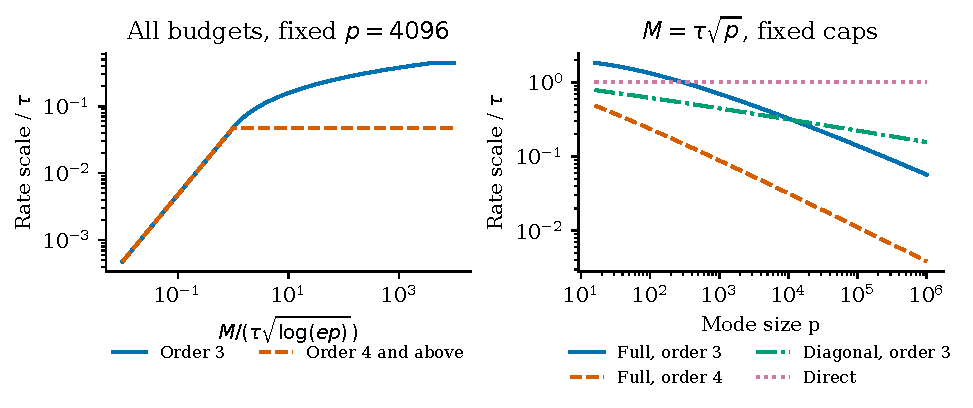
\includegraphics[width=\textwidth]{../figures/01_final_rates.pdf}
\caption{Final analytic rate scales, with unspecified multiplicative constants set to one. Left: all-budget dependence at $p=4096$. Right: full-data and diagonal-information scales at $M=\tau\sqrt p$. These curves display theorem orders; they are not empirical attainment or leading-constant comparisons.}\label{fig:rates}
\end{figure}

\section{Why the full tensor changes the rate}\label{sec:mechanism}
\subsection{The diagonal benchmark and its limits}
For an orthogonal product loading $L=\sum_{i=1}^m w_iV_i$, with orthonormal mode factors and $\norm w_2=1$, the contractions $d_i=\ip Z{V_i}$ have independent Gaussian errors. Put $q_K=2/K$ and
\[
 J_{\Tu}=\min_k\prod_{l\ne k}\bar r_l,\qquad J_{\TT}=\prod_{k<K}\bar r_k.
\]
Canonical expansions and generalized H\"older give
\begin{equation}\label{eq:compress}
 \sum_i|\ip A{V_i}|^{q_K}\le J^{1-1/K}M^{2/K}.
\end{equation}
For TT, the needed squared-weight identity is a prefix-weight identity; the expanded product terms are not assumed orthogonal. At rank one the diagonal image is exactly an $\ell_{2/K}$ ball. This image identity connects the marginal experiment to \citet{collier2017}; the exponent also appears in tensor norm and factor geometry \citep{friedlandlim2018,fan2023}.

With $\lambda=\tau\sqrt{2\log(2m/\alpha)}$, soft thresholding satisfies, on the simultaneous noise event,
\[
 |\soft_\lambda(a_i+\tau g_i)-a_i|
 \le\min(|a_i|,2\lambda)\le |a_i|^{q_K}(2\lambda)^{1-q_K}.
\]
Consequently the center $\sum_iw_i\soft_\lambda(d_i)$ with radius
$\norm w_\infty J^{1-1/K}M^{2/K}(2\lambda)^{1-2/K}$ is honest. One can deterministically choose the smallest of this radius, the direct Gaussian radius and the valid structural radius. This is an executable conservative interval, requiring only $m$ coordinate entries when the factors are coordinate vectors. Dense contractions have additional input cost.

For rank one and $M=\tau\sqrt p$, the flat-loading diagonal rate is
\[\tau(\lp/p)^{(K-2)/(2K)}.\] This rate is sharp for the marginal experiment, but exceeds the full-data rate in Theorem~\ref{thm:main}. Write $H=|S\cap T|$ for the overlap of two equally sized sparse supports. Diagonal alternatives have inner product proportional to $H$. Tensor product alternatives can have full inner product proportional to $H^K$. Replacing one likelihood overlap by the other would invalidate the lower bound.

\subsection{Residual scans and the norm-budget transition}
For each nonempty coordinate set $S$ of size $s$, choose a finite $1/(2K)$ net of each unit sphere in $\R^S$, with cardinality at most $(1+4K)^s$. Define $N_S(R)$ as the largest absolute contraction of $R$ over products of these net vectors. A union bound gives simultaneous thresholds
\[
 \lambda_s(\alpha)=\tau\sqrt{2\{s\log(ep/s)+Ks\log(1+4K)+\log(2p/\alpha)\}}.
\]
Project the confidence set
\[
 \{B\in\Theta:N_S(Z-B)\le\lambda_{|S|}(\alpha)\text{ for every nonempty }S\}
\]
onto $\psi$, with a fixed singleton convention if empty. This set contains the true mean with probability at least $1-\alpha$.

For two feasible tensors their difference has doubled caps. Write $J_2=J(2\bar r)$, $P_2=2J_2^{(K-1)/2}$ and $Q_2=4J_2^{K/2}$. The deterministic diameter bound is
\begin{equation}\label{eq:diameter}
 |C_F(Z)|\le\min\left\{2h_0,\frac1{\sqrt p}\sum_{s=1}^p
 \min\{P_2M,Q_2\lambda_s(\alpha)\}\,s^{-K/2}\right\},
\end{equation}
where $h_0=M\sqrt{r/p}$ and $r$ is the smallest constrained cap, truncated at $p$. Imposing both constraints before summation is essential. For $K=3$ the scan contribution has a harmonic factor; for $K\ge4$ the corresponding sum converges. Evaluating the split sum gives \eqref{eq:rate}.

The cubic lower bound uses sparse factors with magnitudes proportional to $j^{-1/3}$ on a support of size $m$. With scale $b$, their diagonal target is $bH_m/\sqrt p$, while their tensor norm is bounded by $b\sqrt{27m}$, where $H_m=\sum_{j=1}^m j^{-1}$. Suitable support mixing controls the full Gaussian likelihood second moment. Choosing $m$ within the norm constraint and the indistinguishability constraint recovers the intermediate logarithm as well as the saturated cubic branch. The construction and its hypergeometric overlap bound appear in Supplement Theorem~\ref{S-thm:all_norm_rates} and its proof; these, rather than the diagonal image identity alone, establish full-data optimality.

For squared risk let
\[
 T(R)=\max\bigl(0,\max_{S\ne\varnothing}\{N_S(R)-\lambda_{|S|}(1/8)\}\bigr).
\]
A measurable $\tau$-approximate minimizer of $T(Z-B)$ over $B\in\Theta$ exists by a fixed countable dense sequence. Its excess error can be integrated over the full noise tail. A fixed-confidence midpoint bound would instead leave a possible $\alpha M^2$ contribution, which is not uniform in $M/\tau$. This distinction also explains the scalar-estimation correction in Section~\ref{sec:pointwise}.

\subsection{Comparison with neighboring inference problems}
At $M=\tau\sqrt p$, an honest fixed-radius affine interval on the same rank-one class has radius at least a constant times $\tau$. An arbitrary interval required to be honest on a single-unfolding relaxation likewise has expected length at zero at least order $\tau$ (Supplement Theorems~\ref{S-thm:affine} and~\ref{S-thm:unfolding}). Matricization retains the data; the second comparison enlarges the parameter class over which coverage is required. Neither assertion rules out regular-stratum pointwise gains.

The novelty claim is therefore specific: an ordered residual argument and a full-likelihood harmonic mixture yield the cubic all-budget phase diagram under simultaneous tensor constraints. General nonlinear inference on nonconvex sets and honest-adaptation obstructions are established subjects \citep{cailownonconvex2004,cailow2004,juditskynemirovski2020}. The geometric exponent and the sparse marginal benchmark are also precedents, not separate claims of new general principles.

\section{Computation, growing caps and loading geometry}\label{sec:scope}
\subsection{What is implemented}
The residual projection and minimum-residual estimator are statistical constructions. Finite nets do not make the optimization efficient: the number of support/direction constraints can be exponential, and fitting the nonconvex cap class is a second obstacle. A certified residual fit must return a feasible tensor with objective excess at most $c\tau$ on every observation to inherit the stated squared-risk order. A bound only on successful runs is insufficient. For confidence projection, conservative outer endpoints preserve validity even when the requested endpoint tolerance is not attained; achieved precision must be reported separately. Supplement C1 gives the exact optimization contracts.

\begin{table}[t]\small\centering
\begin{tabularx}{\textwidth}{@{}lYY@{}}\toprule
Procedure & Statistical guarantee & Computational status \\\midrule
Residual scan / fit & Fixed-cap flat-loading minimax length / risk & Ideal global nonconvex optimization; general implementation open.\\
Binary rank-one search & Outer projection for its finite-net confidence set & Implemented for mode size two, low order; exponential benchmark with guarded float64 bounds.\\
Diagonal threshold & Cap-uniform finite-sample coverage & Explicit contractions and thresholding; generally above the full-data minimax rate.\\
Structural/direct selection & Sharp when minimum cap $r\gtrsim\sqrt p$ & $O(p)$ coordinate accesses; dense contraction cost additional.\\
Cap-valid tangent interval & Outer-class honesty; P1 pointwise length under stated conditions & Full-tensor economy SVD and projection, polynomial for fixed order.\\
R1 companion & Uniform noise-scale squared-risk bound & Separate scalar output with constant additional work.\\\bottomrule
\end{tabularx}
\caption{Procedure, guarantee and implementation are kept distinct. Global float64 diagnostics are not formal interval arithmetic. Input storage of a full tensor is $O(p^K)$ even when a coordinate procedure reads only $p$ entries.}\label{tab:methods}
\end{table}

Fixed-depth truncated scans have polynomial cost for fixed order and depth, but leave a nonvanishing gap from the ideal rate in the relevant asymptotic comparison. Low-degree polynomial estimators also have a proved separation from unrestricted squared risk in specified sparse-prior regimes \citep{choo2021}. This is a restriction on a particular estimator class; it is not a lower bound for every polynomial-time interval procedure. A general computational lower bound would require an additional testing hypothesis and reduction.

\subsection{Growing-cap regimes}
\begin{theorem}[Matched large-cap regime]\label{thm:growing}
Let $r=\min(p,\min_k\bar r_k)$ for the constrained unfoldings. For a fixed $c>0$, if $r\ge c\sqrt p$, then for flat loading
\[
 \calL_0\asymp_{\alpha,c}\calL_{\max}\asymp_{\alpha,c}
 \min\{M\sqrt{r/p},\tau\},
 \qquad\mathcal R\asymp_{\alpha,c}\min\{M^2r/p,\tau^2\}.
\]
Constants are independent of growing ranks and order. Deterministic structural/direct selection attains the upper orders.
\end{theorem}
Supplement G1 supplies the proof. Its lower bound mixes $A_S=b\sum_{i\in S}E_i$ over size-$r$ supports, with
\[
 b=\min\{M/\sqrt r,\tau\sqrt{\log(1+p/(4r^2))}\}.
\]
For every $1\le r\le p$, this gives the lower scale
\begin{equation}\label{eq:intermediate}
 \min\left\{M\sqrt{r/p},\frac{\tau r}{\sqrt p}\sqrt{\log(1+p/(4r^2))}\right\}.
\end{equation}
Combining this with the structural/direct upper bound matches when $r\gtrsim\sqrt p$. For $1\ll r\ll\sqrt p$ these envelopes can be far apart. The fixed-cap constants of Theorem~\ref{thm:main} cannot be extrapolated to resolve that gap. The retained intermediate-cap experiments display it as an analytic upper/lower comparison, not evidence for a new exponent.

\subsection{Loading-dependent rates and the unresolved profiles}
For an arbitrary prescribed $L$, let
$\rho(L)=\sup_{\norm{u_k}_2=1}|\ip L{\bigotimes_ku_k}|$ be its product overlap. At fixed positive caps and $M\le\tau$, the minimax length scale is $M\rho(L)$ and squared risk has its square (Supplement L1). Canonical expansions bound the structural functional radius by $\sqrt J M\rho(L)$; a two-point product alternative gives the lower bound. Computing $\rho(L)$ can itself be difficult, so this is not a blanket efficient algorithm.

For an orthogonal product loading with decreasing absolute weights, fixed $\beta>0$ and $C_0<\infty$, assume $|w_i|\le C_0|w_1|i^{-\beta}$. At fixed positive caps and order, Supplement W2 proves, for every budget,
\[
 \calL_0\asymp\calL_{\max}\asymp |w_1|\min(M,\tau),\qquad
 \mathcal R\asymp |w_1|^2\min(M,\tau)^2.
\]
A dyadic block construction yields an upper bound involving
$\sum_j a_j(j+1)^{\nu_K}$, with block maximum $a_j$ and $\nu_3=3/2$, $\nu_K=1/2$ for $K\ge4$. Polynomial decay makes this sum finite relative to $|w_1|$. A product alternative on the largest weight gives the matching lower bound. The upper construction still uses ideal block fits.

Constants deteriorate as $\beta\downarrow0$; dimension-dependent decay approaching zero is not covered uniformly. Known nonorthogonal perturbations $R$ with $\norm R_F\le\epsilon|w_1|$, fixed $\epsilon<1$, retain these orders with a direct residual correction. Completely arbitrary unequal profiles at larger budgets remain unresolved. Flat loadings, fixed decay and small budgets for every loading are different matched regimes, not a complete loading theory.

\section{Adaptation and an executable pointwise result}\label{sec:pointwise}
Positive fixed outer caps allow rate adaptation to smaller positive fixed caps because Theorem~\ref{thm:main} has the same order, with constants allowed to depend on the outer cap. This assertion is neither rank recovery nor uniform adaptation as the outer caps grow. At $M=\tau\sqrt p$ and outer minimum cap $r\gtrsim\sqrt p$, every outer-honest interval has expected length at zero at least order $\tau$. The known fixed-cap oracle rate is $o(\tau)$. Since zero is in every positive inner cap class, simultaneous minimax adaptation across these classes is impossible (Supplement G2). A translated disjoint-block mixture gives a related obstruction at nonzero means when extra weak rank fits within the caps and norm budget.

A different conclusion holds at strong means saturating the supplied Tucker mode caps. The following result does not substitute TT bond caps for Tucker mode caps.
\begin{theorem}[Strong saturated pointwise length]\label{thm:pointwise}
Let all Tucker mode caps equal $r$, and let
$A_0=\sum_{i\in S}a_iE_i$, $|S|=r$, $a=\min_{i\in S}|a_i|>0$.
Assume, for fixed $c_0>1$,
\[
 \norm{A_0}_F+\tau\le M\le c_0a\sqrt r.
\]
Set $v=\sqrt2\tau$, $\delta=\alpha r/(8p)$ and
\[
 \eta=2v\sqrt{2\{(p+p^{K-1})\log9+\log(2K/\delta)\}}.
\]
If $a\ge4\eta$ and $a\ge\eta^2\sqrt p/\tau$, a polynomial interval honest on the entire unseparated Tucker cap class satisfies
\[
 \E_{A_0}|C|\asymp_{K,\alpha,c_0}\tau\sqrt{r/p}.
\]
This matches the best expected length at $A_0$ under the same outer honesty class.
\end{theorem}
The proof is Supplement P1. The support and amplitudes are not supplied to the algorithm. The sufficient amplitude is of order $\tau p^{K-1/2}$ at fixed confidence and order; it is conservative and is not an optimal signal threshold. Norm comparability prevents a loose outer budget from overwhelming the local bias certificate. Saturation removes unused weak rank in the coordinate family. The theorem is a length result, not a pointwise squared-risk theorem.

For clarity, the executable procedure uses an artificial split
$Z^{(1)}=Z+\tau G'$ and $Z^{(2)}=Z-\tau G'$, giving independent errors of scale $v$. Let $Q_k$ be the pilot top-$r$ mode projector and $\widehat s_{kr}$ the pilot $r$th singular value. Set
\[
 e_k=\begin{cases}\min\{1,2\eta/(\widehat s_{kr}-\eta)\},&\widehat s_{kr}>\eta,\\1,&\text{otherwise},\end{cases}
\]
with $e_k=0$ for full mode cap. With an identity in each omitted mode, put
\[
 T_Q=\sum_k\bigotimes_{l\ne k}Q_l-(K-1)\bigotimes_lQ_l,
 \qquad B=M\norm{(I-T_Q)L}_F\min\left\{1,\sqrt{\sum_{k<l}e_k^2e_l^2}\right\}.
\]
Conditional on the pilot, choose the smallest-radius candidate among tangent, split-direct and structural intervals. Their centers are $\ip{T_QL}{Z^{(2)}}$, $\ip L{Z^{(2)}}$, $0$, and their radii are $B+z_{\rm val}v\norm{T_QL}_F$, $z_{\rm val}v$, $h=M\sqrt{r/p}$, where $z_{\rm val}=z_{1-(\alpha/2-\delta)/2}$. Intersect with $[\ip LZ-d,\ip LZ+d]$ and $[-h,h]$, with $d=z_{1-\alpha/4}\tau$, reporting $\{0\}$ if empty. This retains outer-class honesty and bounds length by $2d$ even on pilot failure.

The original implementation also reported the midpoint of this interval as an estimate. A zero sentinel on a rare empty intersection can give an error comparable to the signal itself. The following separate output repairs that defect without changing the reported interval.
\begin{proposition}[R1: scalar companion]\label{prop:companion}
Suppose $Y=\psi+\tau g$, $g\sim N(0,1)$, $|\psi|\le h$, and an arbitrary candidate is intersected with $[Y-d,Y+d]$ and $[-h,h]$, where $d=z_{1-\alpha/4}\tau$. Define $\widehat\psi=0$ if $h\le\tau$. Otherwise use the midpoint of a nonempty intersection and $\Pi_{[-h,h]}Y$ if empty. Then
\[
 \E(\widehat\psi-\psi)^2\le
 \begin{cases}h^2,&h\le\tau,\\
 \tau^2\{1+2z_{1-\alpha/4}\sqrt{2/\pi}+z_{1-\alpha/4}^2\},&h>\tau.
 \end{cases}
\]
Replacing an exactly zero singleton by the same clipped direct estimate is also valid for this scalar output.
\end{proposition}
\begin{proof}
The first branch has error at most $h$. On a nonempty intersection the midpoint differs from $Y$ by at most $d$. Projection onto $[-h,h]$, which contains $\psi$, cannot increase its distance from $\psi$. Thus the second branch has pathwise error at most $\tau|g|+d$. Integrating with $\E g^2=1$ and $\E|g|=\sqrt{2/\pi}$ gives the result. No successful-pilot conditioning or candidate independence is used.
\end{proof}
This bound is uniform over the budget and removes the arbitrary sentinel's $M^2$ loss. It does not establish the ideal weak-signal minimax risk or the smaller P1 pointwise squared-risk rate. For a general prescribed loading use noise scale $\tau\norm L_F$ and a valid structural radius. The public implementation returns the interval and this estimator separately, with the midpoint retained as a diagnostic.

\section{Noise, supplied bounds and calibration}\label{sec:robustness}
The baseline noise model has separate upper- and lower-bound roles. Joint sub-Gaussian directional control permits the residual-scan upper bounds with a known proxy. Marginal coordinate bounds alone do not calibrate all product directions. Gaussian likelihood identities give the lower bounds; a minimax lower bound over a noise family containing Gaussians does not prove an identical lower bound for each fixed non-Gaussian law.

With independent full replicates and a known covariance upper bound, directional block medians yield finite-variance scan bounds when the number of independent replicates exceeds the required scan complexity. Replicate independence is needed for concentration across blocks. Arbitrary dependence cannot be repaired by interpreting the total number of recorded tensors as independent sample size. A simpler coordinate refinement allows a known number $c$ of corrupted whole replicates: choose an odd number of blocks $b>\max\{8c,32\log(m/\alpha)\}$, require $n\ge2b$, and use threshold $\Lambda=2\bar\sigma/\sqrt{\lfloor n/b\rfloor}$. Median contraction errors are then simultaneously bounded with the stated probability (Supplement Proposition~\ref{S-prop:mom}). This is a coordinate-envelope calibration, not a sharp general contamination minimax theorem.

Unknown scale has a finite-sample solution in the independent Gaussian replicate setting. With $m$ orthogonal contractions, $n\ge2$ and residual variance $S^2$, the degrees of freedom are $\nu=m(n-1)$. The bound
\[
 \sigma_U=S\sqrt{\nu/\chi^2_{\nu,\delta}}
\]
is independent of the sample mean and exceeds $\sigma$ with probability $1-\delta$. Conditional interval selection at level $1-\alpha_0$ using $\sigma_U$ is honest unconditionally at least at level $1-\alpha_0-\delta$ (Supplement Proposition~\ref{S-prop:variance}). This argument does not justify a same-data plug-in normal quantile under arbitrary noise.

A supplied Frobenius approximation allowance $\varepsilon_A$ adds its size, up to the direct-noise ceiling, to the flat-loading interval scale; an uncharged loading residual can similarly invalidate coverage. Data-selected loadings are outside the prescribed-loading theory unless selection is made independent or calibrated uniformly. Missing-entry experiments, dependent replicates without a concentration model and fully unknown directional scale remain separate problems. The supplement retains the complete assumptions and counterexamples for these distinctions.

\section{Experiments linked to the guarantees}\label{sec:experiments}
The revision retains the original 1,084,640 saved Monte Carlo datasets and re-evaluates all 303 interval-producing cases under the corrected numerical and scalar definitions; no new noise is drawn for that reevaluation. It adds 87,200 independently seeded datasets across 55 pre-specified configurations. V01 uses 1,000 paired datasets at each of ten signal levels, V02 uses 50 observations at each of four amplitudes shared across three search budgets, V03 uses 1,000 datasets in each of 19 corruption/noise cases, V04 uses 3,000 in each of 18 variance cases, and V05 uses 1,000 in each of four larger pointwise cases. Tables and figures are generated from raw endpoints and estimates. The empirical supplement contains the full configuration registry, paired differences, failures, Wilson coverage intervals, length standard errors and estimator identities.

Coverage comparisons allow only four representable endpoint steps for rounding, retain strict counts, and have no target-scaled statistical tolerance. Re-evaluation changes two 90\% rows for the same observation: the known-noise XCH and oracle counts in S03\_007 change from 134/150 to 133/150. An exact-noise replay distinguishes that genuine miss from the harmless one-ULP structural-boundary discrepancies. Two power-of-two rescalings per saved interval case preserve the revised events. These numerical checks do not constitute formal interval arithmetic.

\paragraph{Supplied budgets and controlled ablations.}
V01 holds the outer budget fixed while varying the signal, with a paired norm-comparable budget branch. All comparisons use the same observation and pilot. Bias-only removal freezes the original candidate choice; fallback-only removal forces the tangent candidate and retains both intersections; quantile-only removal changes only the validation critical value. A separate no-intersection diagnostic and the historical combined diagnostic are also retained. At weak signals, bias-only removal changes no reported interval because the fallback is selected. Thus the old combined failure cannot be attributed to bias alone. Reducing the validation quantile can lower coverage while preserving the other protections.
At amplitude two, fixed-budget cap coverage is 0.960 and the regular XCH comparator has coverage 0.001. At the largest amplitude, cap coverage is 0.966 with mean length 1.936. These are finite-sample observations, not uniform performance guarantees. The norm-comparable sweep answers a different question because its supplied class changes.
\begin{figure}[t]\centering
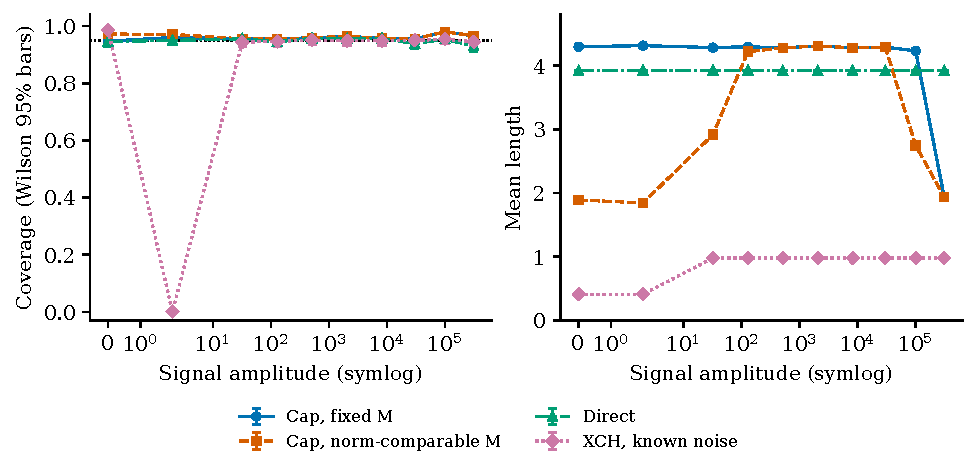
\includegraphics[width=\textwidth]{../figures/02_fixed_budget.pdf}
\caption{Paired fixed-budget and norm-comparable signal sweeps at $p=16$, cap one and $\tau=1$, with 1,000 new datasets per amplitude. The fixed budget is $342023.69$ throughout. Bars are Wilson 95\% coverage intervals or 1.96 standard errors for mean length. XCH is not guaranteed over the weak-signal cap union.}\label{fig:signal}
\end{figure}
\paragraph{Pointwise precision and scalar loss.}
In the four new $p=32,64$ cases, cap coverage ranges from 0.965 to 0.978; normalized mean lengths range from 7.20 to 8.01 times $\tau\sqrt{r/p}$. This supports the stated finite-grid behavior under deliberately strong P1 conditions, without identifying a limiting slope or optimal signal threshold. Regular XCH and the support oracle have smaller constants here.

The saved S03\_002 midpoint MSE is 12,084,661.379, with one sentinel event among 500 draws. The R1 companion on the same observations has MSE 0.148 (standard error 0.025), below its uniform theoretical bound 9.601. All sentinel observations remain in the loss calculation, and every interval endpoint is unchanged. The old midpoint is retained as a diagnostic, never relabeled as the R1 estimator.
\begin{figure}[t]\centering
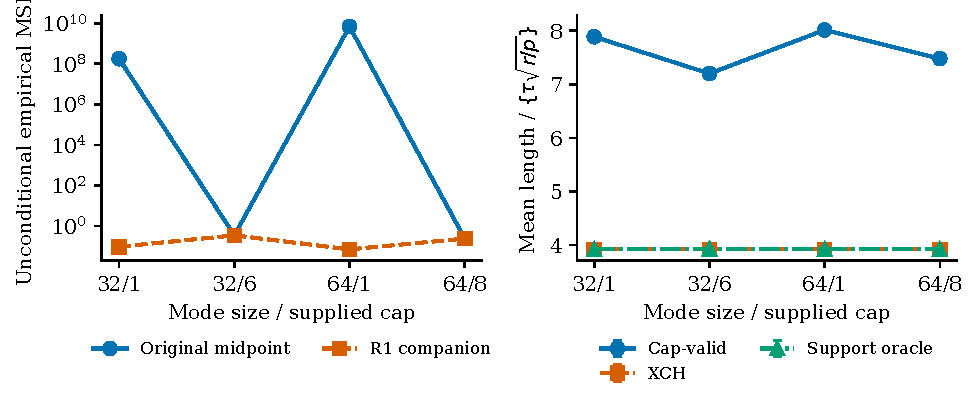
\includegraphics[width=\textwidth]{../figures/04_scalar_and_pointwise.pdf}
\caption{Strong saturated cases with 1,000 new datasets each. Left: unconditional empirical MSE including rare sentinel losses; the scalar correction leaves confidence intervals unchanged. Right: length divided by $\tau\sqrt{r/p}$, with 1.96 standard errors. The logarithmic MSE display does not assert precise estimation of rare-loss expectations; all raw losses and their uncertainty are retained.}\label{fig:pointwise}
\end{figure}
\paragraph{Calibration and assumption violations.}
All 18 within-cap whole-replicate corruption cases have median-interval coverage 1.000 in 1,000 trials each, with conservative lengths; the deliberately violated 120-row/zero-supplied-cap case has coverage 0.000. For $m=1,n=2,\sigma=1$, independent upper-scale calibration has coverage 0.995 versus 0.703 for the naive plug-in. Gaussian residual independence and the chi-square degrees of freedom are part of the experiment, not assumed for arbitrary noise. Fourth-moment-based MSE error bars are not asserted for the heavy-tail cases.

\paragraph{Optimization and input cost.}
V02 fixes the arbitrary loading, signal direction, norm budget, noise and tolerance across all budgets. Of 600 solves, 7 meet endpoint tolerance $0.05$, all at the largest budget and strongest amplitude; 593 remain unresolved. Mean gaps at 3,000 nodes range from 0.127 to 0.353. All feasible-witness gaps are finite and retained, including failures. These guarded float64 outer bounds do not implement the ideal high-dimensional minimax estimator. Fresh timings of the revised public scalar/interval interface use one thread, one warmup and ten calls per dimension; $p=64$ requires 2,097,152 input bytes and averages 0.0876 seconds per call. Traced allocations exclude the preallocated input and potentially untraced native workspace.

The XCH comparison is a local implementation of the tensor-PCA procedure in Section 4.2 of \citet{xu2025}: HOSVD initialization and two simultaneous projection updates, with known-noise and residual plug-in scales. Its regular-stratum theorem requires more than correct rank. Zero and rank-mismatched cases are explicitly outside the specified model; initialization, alignment and remainder constants are not certified for the other individual cases. No inference of finite-sample cap-uniform coverage or leading-constant dominance is made from these comparisons.


\section{Discussion and remaining problems}\label{sec:discussion}
The full tensor contains useful functional information beyond its diagonal marginal even when the class permits arbitrarily weak signals. For flat orthogonal loadings and fixed positive caps, the residual geometry and full-likelihood mixtures determine all-budget minimax rates. The cubic logarithmic transition is the main tensor-specific statistical conclusion. The rank-one image identity, soft-thresholding benchmark and generic adaptation logic have classical antecedents and are not presented as new general principles.

Four substantial extensions remain. First, no general efficient optimizer is implemented or proved minimax for the original fixed-cap diffuse-loading weak-signal class. The binary search illustrates a rigorous real-arithmetic contract with numerical bounds, not a scalable resolution. Second, intermediate growing caps can leave a substantial gap between \eqref{eq:intermediate} and available upper bounds. Third, arbitrary loading profiles beyond the matched flat, fixed-decay and small-budget regimes lack a complete sharp theory. Fourth, P1 covers strong saturated coordinate Tucker means with a norm-comparable outer class; complete pointwise geometry, optimal signal thresholds, nonsaturated means and TT-specific pointwise results are open. General growing-cap adaptation is already impossible in the stated G2 comparison, so a universal positive adaptation theorem would be false.

The new scalar companion supplies noise-scale risk control with unchanged intervals. Its simplicity should not be mistaken for pointwise minimax squared risk. The simulations reveal conservative constants, sensitivity to supplied budgets, weak-signal failure of out-of-domain regular comparators, and unresolved optimization gaps. Full-tensor SVD computation costs $O(Kp^{K+1})$ arithmetic with $O(p^K+p^2)$ working storage at fixed order; diagonal coordinate access and dense rotated contraction costs must be reported separately.

This is a theory and simulation paper. No repeated-tensor application with a defensible independent sampling unit and prescribed contrast was established in the available project materials. A real-data study should identify that unit, dependence structure, noise calibration and norm/cap justification before attaching practical interpretation to these intervals. Neither empirical success on simulated cases nor a broader robustness paragraph substitutes for those requirements.

\bibliographystyle{plainnat}\bibliography{references}
\end{document}
